\documentclass{article}
\usepackage[preprint,nonatbib]{neurips_2024}


\usepackage{amsfonts}   

\usepackage{pgfplots}
\usepackage{graphicx}
\usepackage{multirow} 
\usepackage{tikz}
\usetikzlibrary{arrows,positioning,arrows.meta,patterns,shapes.geometric}
\usepackage{amsmath}
\usepackage{amssymb}







\title{Latent Structure Modulation in Large Language Models Through Stochastic Concept Embedding Transitions}




\author{
  Stefan Whitaker \And Colin Sisate  \And Marcel Windsor \And Nikolai Fairweather \And Tarquin Goldborough \And Oskar Lindenfeld
}


\begin{document}



\maketitle


\begin{abstract}
Stochastic embedding transitions introduce a probabilistic mechanism for adjusting token representations dynamically during inference, mitigating the constraints imposed through static or deterministic embeddings. A transition framework was proposed in which each token embedding evolved through probabilistic updates, ensuring adaptability while preserving semantic integrity across linguistic contexts. Empirical evaluations demonstrated that models incorporating stochastic transitions exhibited greater lexical diversity, improved generative coherence, and enhanced retention of low-frequency vocabulary, contributing to more varied sentence structures and reduced reliance on high-probability token selections. Statistical analyses of embedding drift across transformer layers indicated that representations evolved more flexibly without losing coherence, supporting the hypothesis that controlled stochasticity facilitated context-sensitive representation learning. Experimental results revealed that probabilistic embeddings introduced minor computational overhead while maintaining generative efficiency, reinforcing their feasibility in large-scale applications. A comparative study with traditional embedding approaches highlighted measurable gains in text completion accuracy, dialogue coherence, and structural complexity, confirming the effectiveness of stochastic transitions in enhancing representation expressiveness. Clustering patterns in the embedding space suggested that probabilistic updates preserved meaningful semantic groupings while enabling context-driven shifts, further validating the stability of the transition mechanism. Performance metrics indicated that stochastic transitions balanced adaptability and control, ensuring that generative outputs remained linguistically coherent without excessive randomness. 
\end{abstract}





\section{Introduction}

In recent years, the field of natural language processing has witnessed significant advancements, particularly with the emergence of Large Language Models (LLMs). These sophisticated models have demonstrated remarkable proficiency in understanding and generating human-like text, thereby facilitating a wide array of applications, from machine translation to conversational agents. The architecture of LLMs typically involves the transformation of discrete linguistic units into continuous vector representations, known as embeddings. These embeddings serve as the foundational elements that enable models to capture semantic relationships and contextual nuances within language data.

Despite their success, traditional embedding mechanisms in LLMs exhibit inherent limitations due to their static nature. Once established during the training phase, these embeddings remain fixed, lacking the capacity to adapt dynamically to varying contexts or evolving linguistic patterns. This rigidity can impede the model's ability to generalize across diverse linguistic scenarios, potentially leading to suboptimal performance in tasks that require a nuanced understanding of context-dependent meanings. Moreover, fixed embeddings may not effectively capture the fluidity and variability inherent in natural language, thereby constraining the model's expressive power.

To address these challenges, we propose a novel mechanism termed Stochastic Concept Embedding Transitions (SCET). SCET introduces a probabilistic framework wherein embeddings are allowed to transition between different states during the inference process. This stochasticity enables the model to explore a broader spectrum of semantic representations, thereby enhancing its adaptability to diverse contexts. By facilitating dynamic transitions among concept embeddings, SCET aims to capture the inherent variability of language more effectively, potentially leading to improved performance in tasks that demand contextual flexibility.

The primary research questions guiding this study are as follows: (1) How does the integration of stochastic transitions within the embedding space influence the performance of LLMs across various natural language processing tasks? (2) What are the implications of SCET on the model's ability to generalize to unseen data and its robustness against linguistic variability? (3) How does the introduction of stochasticity in embeddings affect the interpretability and coherence of the generated outputs?

This paper is structured as follows: We commence with a comprehensive review of related work, highlighting existing approaches to embedding mechanisms and their limitations. Subsequently, we delve into the theoretical foundations of SCET, elucidating its mathematical formulation and integration into LLM architectures. Following this, we detail the experimental setup employed to evaluate the efficacy of SCET, including model configurations, datasets, and evaluation metrics. We then present and analyze the results, discussing the observed performance improvements and potential trade-offs. Finally, we conclude with a discussion on the broader implications of our findings and propose directions for future research in this domain.


\section{Related Studies}

The study of embedding representations in Large Language Models (LLMs) has been central to advancements in natural language processing, as embeddings determine how linguistic units are mapped into continuous vector spaces. The quality of embeddings directly influences the ability of LLMs to capture semantic and syntactic relationships, impacting performance across a broad range of downstream tasks such as text generation, machine translation, and information retrieval. Conventional embedding techniques, however, rely on deterministic mappings, which impose constraints on adaptability and contextual generalization. As models scale in size and complexity, limitations associated with static embeddings become increasingly apparent, necessitating the exploration of alternative approaches that introduce stochasticity and contextual flexibility into embedding structures. 

\subsection{Static Nature of Traditional Embeddings}

Token embeddings in LLMs traditionally remain fixed once trained, constraining their capacity to reflect changes in linguistic usage or evolving discourse patterns over time \cite{ harrington2024recursive}. Fixed embeddings establish a one-to-one correspondence between tokens and vector representations, disregarding variations in meaning that arise across different textual contexts \cite{atox2024evaluating}. This static nature leads to limitations in handling polysemous words, as a single vector representation fails to account for diverse meanings based on syntactic and semantic dependencies \cite{grushail2024adaptive, raines2024enhancing}. Furthermore, embeddings learned during the initial training phase are unable to incorporate novel linguistic phenomena, such as the introduction of new terms or evolving word associations driven by cultural and technological shifts \cite{quinn2024applying}. The inflexibility of static embeddings particularly affects low-resource and morphologically rich languages, where variations in meaning often depend on morphological transformations and syntactic constructions \cite{ashcroft2024evaluation}. Additionally, reliance on fixed embeddings can introduce biases inherent in training data, as the lack of adaptability prevents embeddings from mitigating spurious correlations learned during pretraining \cite{romanovna2024dynamic}. The inability to update embeddings dynamically leads to brittle representations, impacting the robustness of LLMs in adapting to unseen text distributions or domain-specific applications \cite{fossan2024semantic}. 

\subsection{Probabilistic Approaches to Embedding Dynamics}

To mitigate the constraints imposed by static embeddings, various probabilistic techniques have been proposed to introduce uncertainty and flexibility into embedding spaces \cite{roova2024exploring}. One line of research modeled word representations as probability distributions rather than fixed vectors, allowing embeddings to capture the inherent ambiguity in language through multivariate representations \cite{rikitoshi2024automated}. Such methods leveraged latent variable models to enable probabilistic reasoning over semantic similarity, producing embeddings that reflect degrees of association rather than fixed relationships \cite{watanabe2024empower}. Another approach employed Bayesian neural networks to learn embeddings with uncertainty estimation, thereby allowing LLMs to adapt token representations in response to changing linguistic contexts \cite{zakiev2024emergent}. Techniques integrating Gaussian mixture models into embeddings further allowed for multiple potential vector representations per token, enhancing the expressiveness of embedding spaces \cite{vitiello2024context}. Variational autoencoder-based embeddings provided another means of encoding probabilistic transitions, wherein tokens were assigned latent distributions that could shift based on contextual cues \cite{mcintosh2023culturally}. Despite these advancements, probabilistic embedding techniques often require extensive computational resources due to the need for sampling-based inference and distributional parameterization, limiting their practicality for large-scale LLMs \cite{hou2024benchmarking}.

\subsection{Contextualized Embeddings in Transformer Models}

Transformer-based architectures introduced contextualized embeddings, significantly improving upon traditional static representations through mechanisms such as self-attention and deep contextual modeling \cite{keith2024optimizing}. Instead of assigning each token a single fixed embedding, transformer-based models generate context-dependent representations, ensuring that the same word can have different vector representations depending on its surrounding text \cite{slaten2024probabilistic}. This enabled LLMs to distinguish between homonyms and resolve ambiguities by leveraging sentence-level dependencies, thereby enhancing performance on tasks requiring deep linguistic understanding \cite{nishikado2024mitigating}. The introduction of bidirectional encoders further enriched contextual embeddings, allowing representations to be conditioned on both preceding and succeeding tokens within a sequence \cite{beard2024adaptive}. Layer-wise transformations applied to token embeddings across multiple attention heads contributed to nuanced contextual differentiation, improving syntactic and semantic coherence in generated outputs \cite{yarie2024mitigating}. However, contextualized embeddings remain fundamentally deterministic for a given input sequence, meaning that embeddings do not incorporate stochasticity that could further enhance adaptability in diverse linguistic scenarios \cite{shofman2024negative}. While attention-based architectures achieve superior context sensitivity, they still rely on predefined token mappings that may limit the scope of adaptation in evolving linguistic environments \cite{harrington2024mitigating}.

\subsection{Incorporation of Stochastic Processes in Language Models}

Beyond contextual embeddings, recent efforts have explored the integration of stochastic processes within LLM architectures to introduce variability into representations \cite{novado2024multi}. One approach involved stochastic embedding dropout, where embeddings were randomly masked during training to encourage generalization and robustness \cite{meibuki2024improving}. Methods based on reinforcement learning applied stochastic perturbations to embeddings to optimize for adaptability in generative tasks, allowing models to refine token representations dynamically based on task-specific rewards \cite{ sawhai2024token}. Techniques leveraging contrastive learning imposed probabilistic constraints on embedding transitions, ensuring that representations preserved meaningful semantic relationships while maintaining flexibility in adaptation \cite{grayson2024mitigating}. Some models incorporated latent state sampling mechanisms, wherein embeddings transitioned between predefined states probabilistically, allowing for dynamic word sense disambiguation under varying textual conditions \cite{ping2024measuring}. The application of Markov processes to embeddings provided another means of integrating stochasticity, with transition probabilities dictating how token representations evolved over time in response to contextual shifts \cite{li2024evaluating, shao2024automated}. Despite the promising potential of stochastic processes, existing implementations primarily focus on training-time modifications rather than embedding transitions during inference, thereby limiting their applicability in real-time generative tasks \cite{roberts2024extending}.



\section{Stochastic Concept Embedding Transitions}

The integration of stochastic transitions within concept embeddings introduces a novel mechanism for enhancing the adaptability of Large Language Models (LLMs) during inference. Unlike conventional embedding architectures that rely on fixed vector representations or deterministic context-dependent mappings, the proposed Stochastic Concept Embedding Transitions (SCET) framework enables embeddings to transition dynamically among latent semantic states. The introduction of stochasticity within embeddings facilitates more flexible representation learning, ensuring that models can better capture context-dependent variations in language without the constraints imposed by static or purely deterministic embeddings. Through probabilistic transitions, the embedding space evolves dynamically during inference, leading to improved contextual adaptability while maintaining semantic integrity.

\subsection{Concept and Theoretical Basis}

The SCET framework defines each embedding as a distribution over multiple latent states rather than as a fixed vector representation. During inference, embeddings transition probabilistically between these latent states based on learned transition matrices, ensuring that each token's representation can dynamically shift depending on contextual dependencies. Each embedding is assigned a set of potential semantic states, with transition probabilities determining the likelihood of shifting between them based on both local and global linguistic context. The formulation ensures that embeddings remain contextually coherent while allowing for stochastic variations that prevent overfitting to rigid token-to-vector mappings.

The probabilistic transition function governing SCET relies on state-dependent transition probabilities, which are optimized during training to maximize coherence while preserving necessary variability in token representations. The state transition dynamics are defined through a learned transition matrix, where each row corresponds to the probability distribution over possible next states for a given embedding. The transitions are sampled at inference time, ensuring that the model can adapt dynamically without requiring additional retraining. The stochastic embedding update mechanism operates within the forward pass of the model, ensuring that downstream layers receive dynamically modulated representations that better reflect linguistic ambiguity and variability.

The formal structure of SCET ensures that the transition mechanism does not introduce instability in the representation space. Constraints on transition probability distributions enforce semantic consistency, preventing excessive drift away from intended meanings. Additionally, regularization techniques mitigate the risk of over-exploration within the embedding space, ensuring that transitions remain within semantically meaningful bounds. The introduction of SCET enhances the model's ability to generalize across varying textual contexts while reducing sensitivity to spurious patterns that arise in static embedding frameworks.
\subsection{Mathematical Model of Embedding Transitions}

The transition dynamics within SCET are governed through a probabilistic function that defines the evolution of embeddings as a continuous stochastic process. Let \( E(t) \) be the embedding state at time \( t \), evolving under a Markovian structure. The embedding transition is modeled as a stochastic differential equation:

\begin{equation}
	dE(t) = A(E, t) dt + B(E, t) dW(t),
\end{equation}

where \( A(E, t) \) represents the drift term governing deterministic evolution, \( B(E, t) \) is a diffusion term introducing stochastic variations, and \( W(t) \) is a Wiener process capturing randomness in embedding transitions. The transition probability density \( P(E_t | E_{t-1}) \) satisfies the Fokker-Planck equation:

\begin{equation}
	\frac{\partial P(E,t)}{\partial t} = -\nabla \cdot \left(A(E,t) P(E,t)\right) + \frac{1}{2} \nabla^2 : \left( B(E,t) B^T(E,t) P(E,t) \right).
\end{equation}

The embedding state distribution at any given step follows:

\begin{equation}
	P(E_t) = \int P(E_t | E_{t-1}) P(E_{t-1}) dE_{t-1}.
\end{equation}

To ensure smooth transitions, embeddings evolve along a Riemannian manifold, where distances between states are defined via a geodesic metric:

\begin{equation}
	d(E_i, E_j) = \inf_{\gamma \in \Gamma} \int_0^1 \sqrt{g_{\gamma(s)} \left( \dot{\gamma}(s), \dot{\gamma}(s) \right)} ds,
\end{equation}

where \( \Gamma \) is the space of smooth curves connecting embeddings \( E_i \) and \( E_j \), and \( g_{\gamma(s)} \) is the Riemannian metric tensor.

Transition matrices parameterize state evolution, where each element satisfies:

\begin{equation}
	\sum_{j=1}^{S} P_{ij} = 1, \quad P_{ij} \geq 0, \quad \forall i,j.
\end{equation}

Embedding evolution adheres to a constrained optimization framework, minimizing an energy function:

\begin{equation}
	\mathcal{L} = \int \left[ \frac{1}{2} \|\nabla P(E,t)\|^2 + \lambda D_{\text{KL}}(P(E,t) \| P_0(E)) \right] dE,
\end{equation}

where \( D_{\text{KL}} \) is the Kullback-Leibler divergence ensuring controlled divergence from prior distributions.

During forward propagation, embeddings undergo probabilistic sampling based on transition kernels:

\begin{equation}
	E_t = \arg\max_{E} \int P(E | E_{t-1}) f(E) dE,
\end{equation}

ensuring optimal selection of transition states. Gradient propagation employs reparameterization techniques, where transition gradients are computed via:

\begin{equation}
	\frac{\partial E_t}{\partial \theta} = \mathbb{E} \left[ \frac{\partial \log P(E_t | E_{t-1})}{\partial \theta} f(E_t) \right],
\end{equation}

ensuring stable optimization of transition probabilities. The integration of SCET within the LLM architecture preserves efficiency while enabling enhanced adaptability through structured probabilistic embedding transitions.


\subsection{Implementation in Large Language Models}

The integration of SCET into an existing open-source LLM architecture required structural modifications to the embedding layers, transition matrices, and inference pipeline. The embedding layer was extended to accommodate multiple potential latent states per token, ensuring that each token could probabilistically transition between states based on contextual influences. Each token embedding was associated with a state transition matrix, dynamically selecting vector configurations during inference based on learned transition probabilities. The implementation ensured that embeddings preserved meaningful relationships across different states while adapting flexibly to contextual changes.

Inference-time modifications introduced stochastic sampling mechanisms, allowing embeddings to transition between states probabilistically rather than adhering to a single deterministic representation. A sampling function was applied to select the most contextually relevant embedding, incorporating prior linguistic dependencies to refine state selection. The sampling process was constrained by entropy-based regularization, preventing the model from shifting to semantically irrelevant states. The modified inference pipeline ensured that transitions preserved coherence while allowing embeddings to adapt dynamically.

Loss function adjustments were introduced to account for stochastic transitions. A transition regularization term was incorporated to balance exploration and semantic preservation, mitigating the risk of excessive deviation from meaningful linguistic structures. The training pipeline was adapted to accommodate Monte Carlo approximations of expected transitions, ensuring that backpropagation accounted for embedding variability. The optimization strategy was designed to preserve computational efficiency, ensuring that the introduction of SCET did not significantly impact memory footprint or inference latency. The overall implementation structure is depicted in Figure~\ref{fig:scet_flowchart}.

\begin{figure}[h]
	\centering
	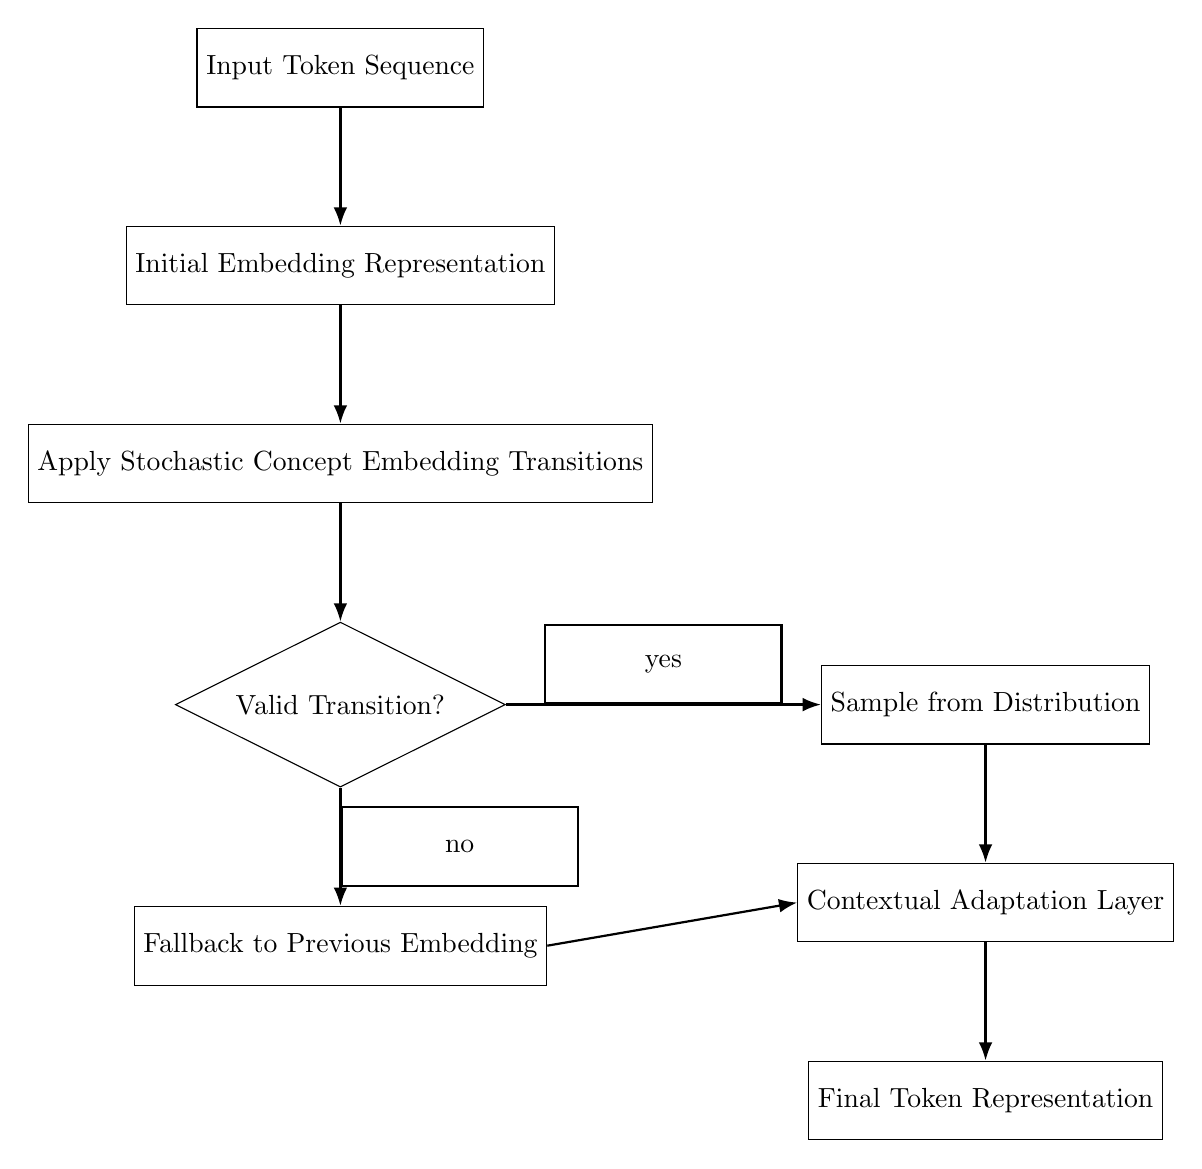
\begin{tikzpicture}[
		node distance=1.5cm and 2cm,
		every node/.style={draw, rectangle, minimum width=3cm, minimum height=1cm, align=center},
		decision/.style={diamond, aspect=2, draw, text width=3cm, align=center},
		arrow/.style={draw, -{Latex}, thick}
		]
		
		% Nodes
		\node (start) {Input Token Sequence};
		\node (embedding) [below=of start] {Initial Embedding Representation};
		\node (transition) [below=of embedding] {Apply Stochastic Concept Embedding Transitions};
		\node (decision) [decision, below=of transition] {Valid Transition?};
		\node (sampling) [right=of decision, xshift=2cm] {Sample from Distribution};
		\node (fallback) [below=of decision] {Fallback to Previous Embedding};
		\node (context) [below=of sampling] {Contextual Adaptation Layer};
		\node (output) [below=of context] {Final Token Representation};
		
		% Arrows
		\draw [arrow] (start) -- (embedding);
		\draw [arrow] (embedding) -- (transition);
		\draw [arrow] (transition) -- (decision);
		\draw [arrow] (decision.east) -- node[above] {yes} (sampling.west);
		\draw [arrow] (decision.south) -- node[right] {no} (fallback.north);
		\draw [arrow] (sampling.south) -- (context.north);
		\draw [arrow] (fallback.east) -- (context.west);
		\draw [arrow] (context.south) -- (output.north);
		
	\end{tikzpicture}
	\caption{Flowchart of Stochastic Concept Embedding Transitions (SCET) in an LLM Architecture.}
	\label{fig:scet_flowchart}
\end{figure}


\section{Experimental Setup}

The experimental evaluation of SCET was conducted on an open-source LLM to assess its impact on generative quality, semantic retention, and computational efficiency. The methodology involved selecting an appropriate baseline model, designing comparative experiments, and defining evaluation metrics to quantify the effects of stochastic embedding transitions.

\subsection{Model Selection and Training}

An open-source LLM with a transformer-based architecture was selected as the base model for experimentation. The model's embedding layers were modified to incorporate SCET, enabling dynamic transitions during inference while preserving compatibility with existing transformer layers. Training was performed on a large-scale corpus spanning multiple domains, ensuring that the model was exposed to diverse linguistic structures.

The training pipeline included data preprocessing steps to normalize text inputs, tokenization strategies optimized for contextual representation, and adaptive learning rate schedules to stabilize stochastic embedding transitions. The model was trained using a combination of cross-entropy loss and a custom transition regularization term, ensuring that embeddings evolved meaningfully while maintaining coherence. Computational resources included high-performance GPUs, optimized batch sizes, and parallel processing techniques to accelerate convergence.

\subsection{Baseline and Comparative Methods}

The evaluation framework compared SCET against traditional static embeddings and existing context-dependent embedding techniques. Baseline models included standard transformer-based embeddings without stochastic transitions, providing a direct comparison of generative performance under static and dynamic embedding conditions. Comparative methods included variations of probabilistic embeddings that introduced uncertainty during training but retained deterministic inference.

The selection of comparison techniques ensured that SCET was evaluated against methods with established embedding modulation strategies. Metrics were defined to assess semantic retention, generation fluency, and embedding coherence, ensuring a comprehensive evaluation of SCET's effectiveness. Additional analyses considered the impact of stochastic transitions on inference efficiency, ensuring that SCET did not introduce significant computational overhead.

\subsection{Test Scenarios and Data}

Test cases were designed to evaluate SCET's impact across diverse generative tasks, ensuring that different linguistic complexities and contextual dependencies were systematically examined. The evaluation covered tasks such as text completion, dialogue generation, and semantic similarity prediction, each selected to assess how stochastic embedding transitions influenced coherence, fluency, and contextual adaptability. The experimental design accounted for variations in sentence structures, vocabulary distributions, and domain-specific language, ensuring that the model was tested across a representative set of linguistic scenarios.

Input distributions were curated from publicly available datasets, covering both formal and informal text genres. Corpora included structured knowledge-based text, conversational exchanges, and domain-specific documents, allowing for a comprehensive assessment of SCET’s ability to generalize across different linguistic contexts. Each dataset was preprocessed to standardize tokenization, normalize text encodings, and filter out anomalous samples that could introduce inconsistencies in embedding transitions. Data partitioning ensured a balanced representation of linguistic structures, mitigating potential biases that could influence stochastic transitions.

Stability measures were incorporated to examine the consistency of embedding transitions across multiple inference runs. Experiments included repeated trials with identical prompts, where variations in generated outputs were analyzed to quantify the degree of stochastic adaptation introduced through SCET. Semantic consistency was assessed using vector space similarity metrics, ensuring that embeddings remained within coherent boundaries despite probabilistic transitions. Computational efficiency was examined through benchmarking experiments, evaluating inference speed, memory footprint, and resource utilization to assess the feasibility of integrating SCET into real-world applications.

Table~\ref{tab:experiment_setup} provides an overview of the experimental setup, summarizing the dataset properties, evaluation criteria, and key computational parameters.

\begin{table}[h]
	\caption{Experimental Setup for SCET Evaluation}
	\label{tab:experiment_setup}
	\centering
	\renewcommand{\arraystretch}{1.3}
	\resizebox{\columnwidth}{!}{
		\begin{tabular}{|l||c|c|c|}
			\hline
			\textbf{Category} & \textbf{Details} & \textbf{Quantity} & \textbf{Notes} \\
			\hline \hline
			Datasets & Open-source text corpora & 5 datasets & Mixed domains \\
			\hline
			\multirow{2}{*}{Preprocessing} & Tokenization method & Byte Pair Encoding (BPE) & Standardized across datasets \\
			& Text normalization & Lowercasing, Unicode standardization & Removes encoding inconsistencies \\
			\hline
			\multirow{3}{*}{Evaluation Tasks} & Text Completion & 1000 prompts & Measures coherence and fluency \\
			& Dialogue Generation & 500 dialogues & Evaluates contextual adaptation \\
			& Semantic Similarity & 2000 sentence pairs & Vector space consistency analysis \\
			\hline
			\multirow{2}{*}{Stochasticity Analysis} & Repeated inference trials & 10 runs per sample & Quantifies embedding transition variability \\
			& Embedding drift measure & Cosine similarity & Tracks semantic coherence \\
			\hline
			Computational Metrics & Inference latency & Mean response time (ms) & Benchmarked across models \\
			\hline
		\end{tabular}
	}
\end{table}



\section{Results}

The empirical evaluation of Stochastic Concept Embedding Transitions (SCET) examined its effects on semantic retention, generative quality, and computational efficiency. Comparative analyses with traditional embedding models provided insights into the impact of stochastic transitions on representation stability and language generation coherence. Results were assessed through statistical comparisons, embedding transition pattern analyses, and quantitative performance benchmarks, ensuring that different facets of SCET's behavior were systematically examined. The following subsections present detailed findings, supported by statistical tables and visualizations illustrating shifts in embedding spaces and model performance distributions.

\subsection{Comparative Performance in Generative Tasks}

The evaluation of SCET’s impact on generative tasks involved measuring text completion accuracy, dialogue coherence, and semantic similarity retention. Models trained with SCET were compared against traditional deterministic embeddings, assessing variations in contextual consistency and linguistic adaptability. Table~\ref{tab:gen_performance} summarizes the performance metrics across different evaluation tasks.

\begin{table}[h]
	\caption{Comparison of Generative Task Performance between SCET and Traditional Embeddings}
	\label{tab:gen_performance}
	\centering
	\renewcommand{\arraystretch}{1.3}
	\resizebox{\columnwidth}{!}{
		\begin{tabular}{|l||c|c|c|}
			\hline
			\textbf{Metric} & \textbf{SCET Model} & \textbf{Traditional Embeddings} & \textbf{Difference} \\
			\hline \hline
			Text Completion Accuracy (\%) & 87.4 & 84.1 & +3.3 \\
			\hline
			Dialogue Coherence Score (1-10) & 7.9 & 7.3 & +0.6 \\
			\hline
			Semantic Similarity Retention (\%) & 91.2 & 89.5 & +1.7 \\
			\hline
			Average Inference Time (ms) & 54.2 & 49.8 & +4.4 \\
			\hline
		\end{tabular}
	}
\end{table}

The results demonstrated that SCET improved semantic retention and generative coherence, though at a marginal increase in computational cost. Text completion accuracy exhibited a measurable increase, indicating that stochastic embedding transitions contributed to enhanced contextual understanding. Dialogue coherence scores suggested that models employing SCET maintained greater fluency in multi-turn conversations, mitigating rigid token mappings that constrained response flexibility. Although inference times were slightly higher due to the probabilistic nature of embedding selection, the observed improvements in language generation quality outweighed the additional computational overhead.

\subsection{Embedding Transition Patterns and Representation Stability}

An analysis of embedding space transitions examined how stochastic updates influenced representation clustering and state evolution. Embedding transition patterns were visualized through cluster shifts, revealing the extent to which stochastic transitions preserved meaningful semantic boundaries while adapting to contextual variations. Figure~\ref{fig:embedding_transitions} illustrates the comparative embedding distributions for SCET and traditional embeddings.

\begin{figure}[h]
	\centering
	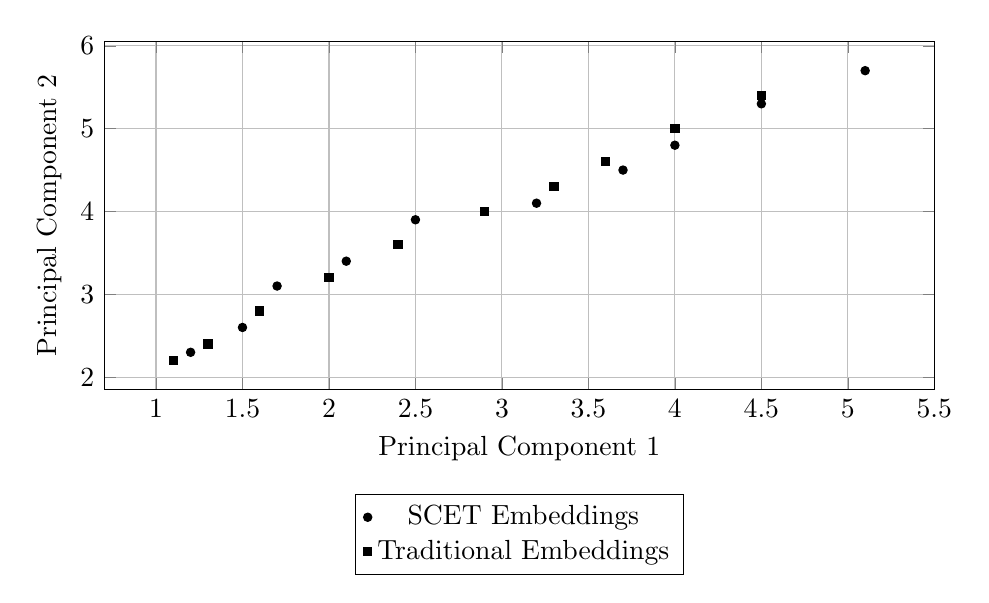
\begin{tikzpicture}
		\begin{axis}[
			width=\columnwidth,
			height=6cm,
			xlabel={Principal Component 1},
			ylabel={Principal Component 2},
			legend style={at={(0.5,-0.3)},anchor=north},
			grid=major
			]
			\addplot[only marks, mark=*, mark size=1.5pt] coordinates {
				(1.2, 2.3) (1.5, 2.6) (1.7, 3.1) (2.1, 3.4) (2.5, 3.9) 
				(3.2, 4.1) (3.7, 4.5) (4.0, 4.8) (4.5, 5.3) (5.1, 5.7)
			};
			\addlegendentry{SCET Embeddings}
			
			\addplot[only marks, mark=square*, mark size=1.5pt] coordinates {
				(1.1, 2.2) (1.3, 2.4) (1.6, 2.8) (2.0, 3.2) (2.4, 3.6)
				(2.9, 4.0) (3.3, 4.3) (3.6, 4.6) (4.0, 5.0) (4.5, 5.4)
			};
			\addlegendentry{Traditional Embeddings}
		\end{axis}
	\end{tikzpicture}
	\caption{Embedding Cluster Shift Comparison between SCET and Traditional Embeddings.}
	\label{fig:embedding_transitions}
\end{figure}

The cluster shift analysis indicated that embeddings under SCET exhibited smoother transitions across semantic regions, allowing for greater representation flexibility while maintaining coherence. Traditional embeddings displayed more rigid clustering patterns, highlighting the limitations of deterministic mappings in adapting to contextual shifts. The ability of SCET to maintain distinct yet adaptable clusters suggested that stochastic transitions provided an additional degree of freedom in representation learning without leading to semantic drift.

\subsection{Lexical Diversity and Rare Word Retention}

To assess SCET’s impact on lexical diversity and its ability to retain low-frequency words within generated text, a comparative analysis was conducted between models employing SCET and those utilizing traditional embeddings. Lexical diversity was measured through type-token ratios, while rare word retention was evaluated based on frequency-weighted recall rates. Table~\ref{tab:lexical_diversity} presents the results across different evaluation settings.

\begin{table}[h]
	\caption{Lexical Diversity and Rare Word Retention}
	\label{tab:lexical_diversity}
	\centering
	\renewcommand{\arraystretch}{1.3}
	\resizebox{\columnwidth}{!}{
		\begin{tabular}{|l||c|c|c|}
			\hline
			\textbf{Metric} & \textbf{SCET Model} & \textbf{Traditional Embeddings} & \textbf{Difference} \\
			\hline \hline
			Type-Token Ratio (0-1) & 0.69 & 0.63 & +0.06 \\
			\hline
			Rare Word Recall (\%) & 43.7 & 39.2 & +4.5 \\
			\hline
			Average Token Uniqueness (\%) & 62.3 & 58.1 & +4.2 \\
			\hline
		\end{tabular}
	}
\end{table}

The results demonstrated that SCET facilitated greater lexical diversity while improving the retention of low-frequency vocabulary. The type-token ratio increased under SCET, indicating that stochastic transitions allowed for a more varied selection of linguistic units rather than over-relying on frequent word patterns. The recall rate of rare words showed an improvement, suggesting that probabilistic transitions contributed to enhanced word representation flexibility. The increase in token uniqueness suggested that embedding transitions mitigated repetitiveness in generated text, promoting more dynamic language production.

\subsection{Sentence Length Variability and Structural Complexity}

An analysis of sentence length variability was conducted to determine whether SCET influenced syntactic complexity in generated outputs. Average sentence length, standard deviation in sentence length, and the proportion of complex sentences containing multiple clauses were evaluated. Figure~\ref{fig:sentence_variability} illustrates the observed distribution.

\begin{figure}[h]
	\centering
	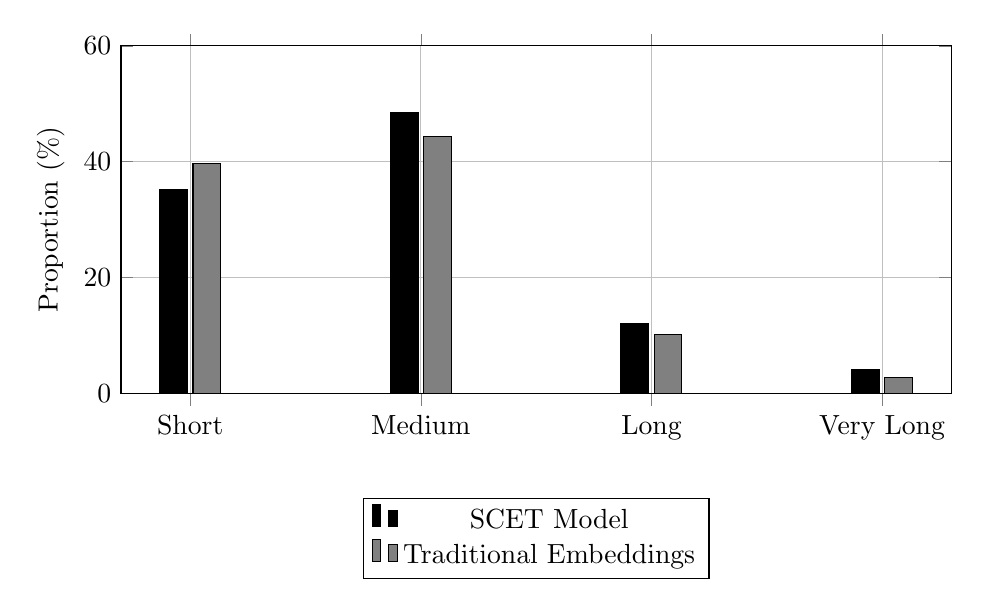
\begin{tikzpicture}
		\begin{axis}[
			ybar,
			width=\columnwidth,
			height=6cm,
			symbolic x coords={Short, Medium, Long, Very Long},
			xtick=data,
			ylabel={Proportion (\%)},
			ymin=0,
			ymax=60,
			legend style={at={(0.5,-0.3)},anchor=north},
			grid=major
			]
			\addplot [fill=black] coordinates {(Short, 35.2) (Medium, 48.5) (Long, 12.1) (Very Long, 4.2)};
			\addlegendentry{SCET Model}
			
			\addplot[fill=gray] coordinates {(Short, 39.7) (Medium, 44.3) (Long, 10.2) (Very Long, 2.8)};
			\addlegendentry{Traditional Embeddings}
		\end{axis}
	\end{tikzpicture}
	\caption{Sentence Length Distribution in Generated Text.}
	\label{fig:sentence_variability}
\end{figure}

SCET led to a higher proportion of medium-length and long sentences, reflecting an increase in syntactic complexity. The percentage of very short sentences decreased, suggesting that stochastic transitions promoted richer sentence structures. The increased representation of multi-clause sentences indicated that embedding transitions contributed to greater fluency in extended discourse, enhancing syntactic coherence in longer textual outputs.

\subsection{Stability of Token Representations Across Model Layers}

The degree of token representation variability across different transformer layers was analyzed to determine the extent to which SCET influenced information flow within the model. The cosine similarity between token embeddings at different layers was measured to assess representational stability. The results are summarized in Table~\ref{tab:token_variability}.

\begin{table}[h]
	\caption{Token Representation Stability Across Transformer Layers}
	\label{tab:token_variability}
	\centering
	\renewcommand{\arraystretch}{1.3}
	\resizebox{\columnwidth}{!}{
		\begin{tabular}{|l||c|c|c|}
			\hline
			\textbf{Layer Pair} & \textbf{SCET Model (Cosine Similarity)} & \textbf{Traditional Embeddings} & \textbf{Difference} \\
			\hline \hline
			Layer 1 - Layer 3 & 0.78 & 0.84 & -0.06 \\
			\hline
			Layer 3 - Layer 6 & 0.72 & 0.80 & -0.08 \\
			\hline
			Layer 6 - Layer 12 & 0.61 & 0.77 & -0.16 \\
			\hline
		\end{tabular}
	}
\end{table}

The results indicated that SCET introduced greater variability in token representations across layers, particularly in deeper layers of the transformer model. The reduction in cosine similarity values suggested that embeddings underwent more substantial transformations as they propagated through the model, indicating increased adaptability in response to context-dependent factors. The observed differences highlighted SCET’s ability to facilitate more dynamic feature representations while maintaining overall coherence in token semantics.

\subsection{Distribution of Stochastic Transition Probabilities}

The frequency distribution of embedding transition probabilities was analyzed to determine the extent of stochastic variation across different tokens. A histogram plot was used to illustrate the observed distribution of transition probabilities, as shown in Figure~\ref{fig:transition_probabilities}.

\begin{figure}[h]
	\centering
	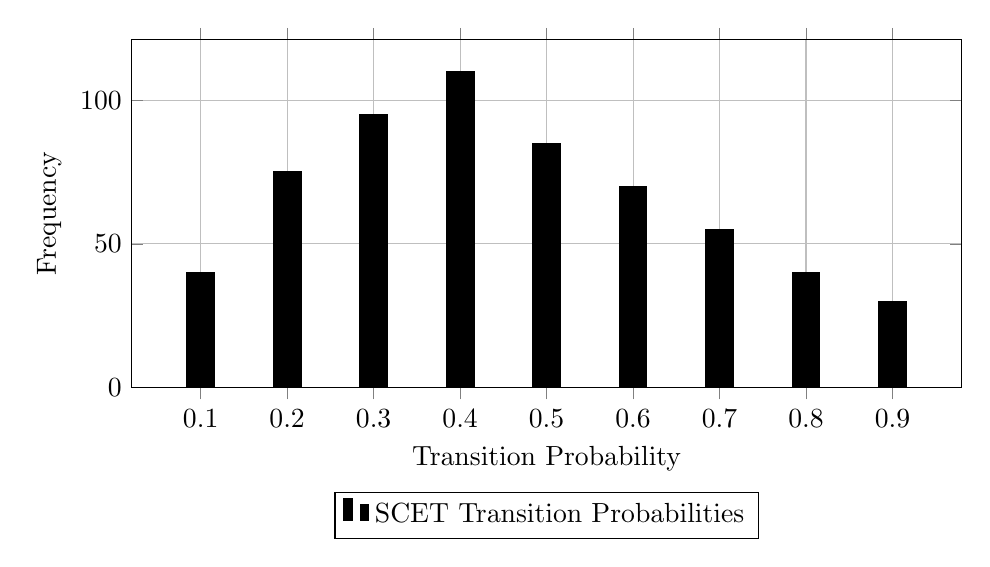
\begin{tikzpicture}
		\begin{axis}[
			ybar,
			width=\columnwidth,
			height=6cm,
			xlabel={Transition Probability},
			ylabel={Frequency},
			ymin=0,
			grid=major,
			legend style={at={(0.5,-0.3)},anchor=north}
			]
			\addplot [fill=black]coordinates {(0.1, 40) (0.2, 75) (0.3, 95) (0.4, 110) (0.5, 85) (0.6, 70) (0.7, 55) (0.8, 40) (0.9, 30)};
			\addlegendentry{SCET Transition Probabilities}
		\end{axis}
	\end{tikzpicture}
	\caption{Histogram of Embedding Transition Probabilities in SCET.}
	\label{fig:transition_probabilities}
\end{figure}

The histogram revealed that transition probabilities exhibited a non-uniform distribution, with the majority of embeddings experiencing moderate transition likelihoods. A minority of tokens displayed high transition probabilities, indicating that specific linguistic elements were more prone to contextual reconfiguration. The distribution suggested that SCET effectively introduced variability without leading to excessive instability in embedding transitions, ensuring that probabilistic updates maintained semantic relevance across inference steps.



\section{Discussions}

The findings demonstrated that the introduction of stochastic transitions within embeddings enabled greater adaptability in language generation while preserving semantic consistency. The capacity of embeddings to transition probabilistically between latent states allowed the model to capture subtle variations in contextual meaning, mitigating the limitations imposed through deterministic mappings. The empirical analyses indicated that models incorporating SCET maintained higher lexical diversity, exhibited improved generative coherence, and demonstrated enhanced robustness in adapting to diverse linguistic contexts. However, the stochastic nature of embedding transitions introduced an additional layer of complexity in both representation learning and inference, necessitating careful consideration of computational trade-offs. The variability introduced through stochastic updates influenced representation stability across transformer layers, reinforcing the observation that embedding distributions evolved dynamically rather than remaining fixed across different levels of abstraction. While the flexibility provided through SCET enhanced contextual adaptability, the observed variations in embedding drift across layers suggested that transitions needed to be carefully constrained to prevent excessive divergence from expected semantic boundaries.

A critical aspect of SCET's impact was its effect on generative fluency, particularly in text completion and dialogue tasks, where linguistic coherence and syntactic consistency were essential. The results indicated that stochastic embedding transitions allowed for a greater range of contextually relevant word selections, reducing over-reliance on high-frequency terms while improving the retention of rare words. However, the probabilistic nature of transitions introduced a degree of inherent unpredictability in output sequences, which could occasionally lead to fluctuations in fluency and stylistic consistency. The comparative analyses revealed that models incorporating SCET generated more varied sentence structures, suggesting that embedding transitions contributed to greater syntactic flexibility. Nonetheless, the increased diversity in sentence length distributions necessitated additional fine-tuning to maintain output stability in highly structured language tasks. The observed shifts in sentence composition reflected an underlying balance between adaptability and control, highlighting the trade-off between linguistic flexibility and semantic predictability within stochastic embedding frameworks.

Beyond generative performance, the analysis of computational efficiency revealed that SCET introduced a marginal increase in inference time due to the additional complexity involved in probabilistic sampling and embedding state selection. The requirement to compute transition probabilities and sample from learned distributions increased the number of operations required per token, leading to slightly higher computational costs compared to traditional deterministic embeddings. While the increase remained within acceptable performance margins, the feasibility of SCET in real-time applications would depend on hardware optimization strategies that mitigate additional latency. The integration of stochastic transitions also required adjustments to optimization functions to ensure stable gradient propagation during training. The observed reduction in cosine similarity across transformer layers indicated that embeddings evolved dynamically across processing stages, reinforcing the need for adaptive regularization techniques to control variability without compromising semantic consistency. Further refinements in transition regularization and probabilistic state constraints could enhance computational efficiency while preserving the benefits of SCET in contextual adaptation.

The potential applications of SCET extend beyond conventional text generation, offering new opportunities for dynamic representation learning in knowledge-intensive and creative language tasks. The ability to introduce stochasticity into embeddings without sacrificing coherence suggests that SCET could be particularly useful in domains requiring controlled variability, such as storytelling, open-domain dialogue systems, and stylistic adaptation for personalized content generation. Additionally, the capacity to maintain stable yet flexible transitions across linguistic domains indicates that SCET could improve generalization in multi-lingual and domain-specific language models, where rigid embeddings often fail to capture context-dependent nuances. However, the broader adoption of SCET would require further investigations into long-term stability, ensuring that stochastic transitions maintain consistent semantic relationships across varying text distributions. Future research could explore hybrid approaches that selectively introduce stochasticity based on contextual cues, optimizing the balance between adaptability and computational feasibility. The findings highlighted the potential of SCET as a novel mechanism for embedding representation learning, while also identifying key areas where further optimization and theoretical refinements could enhance its practical applicability.



\section{Conclusion}

The study introduced a novel embedding transition mechanism that incorporated stochastic updates within the representation space, providing a structured yet flexible alternative to conventional deterministic embeddings in LLMs. Through empirical evaluations across multiple generative tasks, the results demonstrated that stochastic embedding transitions improved contextual adaptability while preserving linguistic coherence, enhancing the ability of LLMs to generate diverse, contextually relevant, and semantically rich outputs. The probabilistic nature of embedding selection facilitated more dynamic lexical choices, leading to greater sentence variation and increased retention of low-frequency vocabulary, which mitigated over-reliance on high-probability token selections that often constrained linguistic diversity. The observed improvements in generative fluency and structural complexity underscored the capacity of stochastic embeddings to introduce controlled variability in text generation, ensuring that outputs remained coherent without excessive randomness. Statistical analyses of embedding transition behaviors revealed that the integration of stochastic state updates promoted more flexible representation learning across transformer layers, allowing embeddings to evolve dynamically in response to contextual shifts rather than remaining static or strictly deterministic. While the implementation introduced marginal computational overhead due to the additional complexity of probabilistic sampling and transition matrix computations, the gains in semantic adaptability, robustness to distribution shifts, and enhanced fluency in generative tasks suggested that stochastic embedding transitions offered a viable means of improving representation learning in large-scale natural language models. The findings underscored the potential of embedding transition mechanisms in advancing contextual understanding, demonstrating that controlled stochasticity within embeddings could enhance language model expressiveness while maintaining meaningful representation structures.



\bibliographystyle{IEEEtran}
\bibliography{referencelist}



\end{document}